% ==============================================================================
\chapter{Thin sensors studies}
\label{ch:ThinSensorsStudies}
%==============================================================================    

\section{Samples and sensors geometries}
Operating conditions for the Timepix3 readout ASICs:
\begin{itemize}
\item I\textsubscript{krum} DAC is set to 10.
\item TOT clock frequency: $40\,\megahertz$
\item VFBK: 150
\end{itemize}
 
\section{Test-beam setup}
\subsection{EUDET telescope ?} 
\subsection{The Timepix3 telescope} \label{sec:Timepix3Telescope}
The Timepix3 telescope is used as a beam reference telescope and is
shown in Figure~\ref{fig:TPX3Telescope}. The telescope is used to
reconstruct the tracks of the particles going through its planes and
extrapolate the position on the Device Under Test (DUT). This allows
to compare the position of the hit on the DUT with the reconstructed
track and calculate the position, time resolutions and the efficiency
of the device. The Timepix3 telescope is made of 6 planes of Timepix3
ASICs~\cite{Timepix3_Poikela} bump bonded to $300\,\micron$ thick
p-in-n planar sensors. The planes are rotated by $9\degrees$ around
the x axis (perpendicular to the beam axis) and the z axis (parallel
to the beam axis) to optimise the charge sharing within the sensors
and obtain a pointing resolution of $\sim$$2\,\micron$ on the device
under test (DUT). The data-driven zero-suppressed mode is used for the
data acquisition of the Timepix3 readout ASICs.

\begin{figure}[htbp]
  \centering
  \begin{tikzpicture}
    \node[anchor=south west,inner sep=0] (image) at
    (0,0){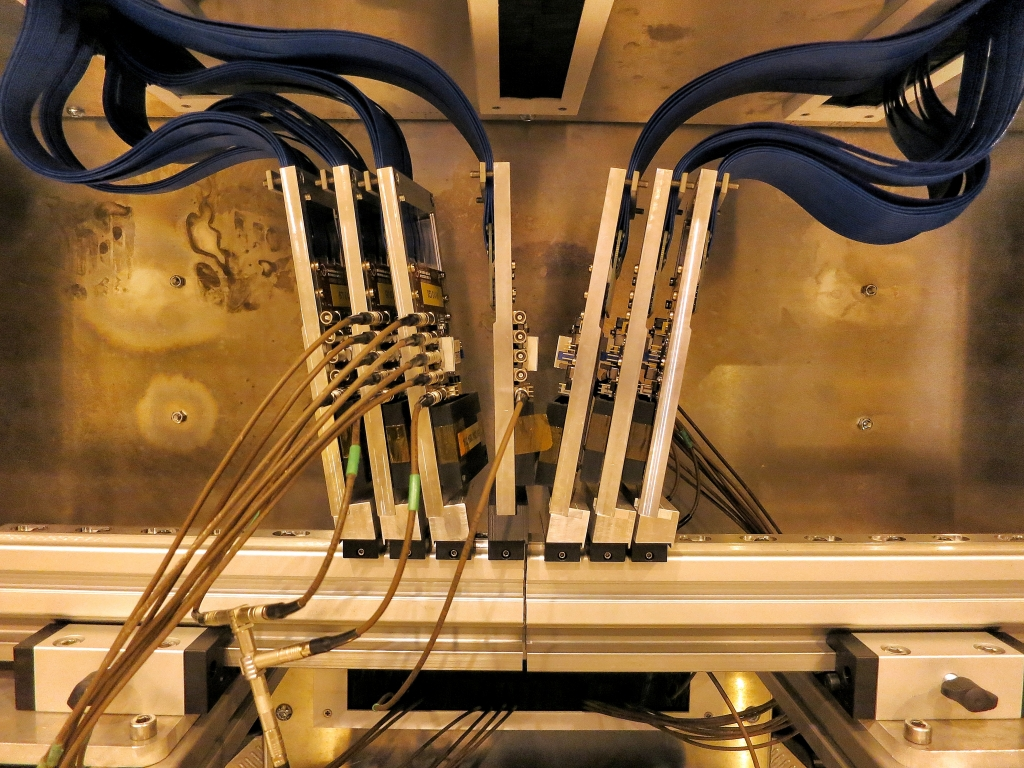
\includegraphics[width=0.6\textwidth]{ActiveEdge/Timepix3Telescope.jpeg}};
    \begin{scope}[x={(image.south east)},y={(image.north west)}]
      \node[above, color=white] at (0.5, 0.85) {Device Under Test};
      \node[above, color=white] at (0.5, 0.78) {(\textbf{DUT})};
    \end{scope}
  \end{tikzpicture} 
  \caption{The Timepix3 beam reference telescope.}
  \label{fig:TPX3Telescope}
\end{figure}

\subsection{Experimental setup at the CERN SPS}
The assemblies are tested at the H6 beam of the CERN SPS using the $120\,\gev$
pion beam. The particle rate obtained per spill is $\sim2.6 \times
10^6$ (UNITS?). The telescope planes were positioned in a way to give
the best tracking resolution for the given beam energy and the level
of multiple scatterings.
For most of the measurements, the DUT is perpendicular
to the beam. A scan was done on the bias voltage and the threshold of
the DUT. The bias scan allows to obtain the depletion voltage.

\section{Reconstruction softwares}
\subsection{EUTelescope}
The EUTelescope software~\cite{Rubinskiy} is used to reconstruct the
telescope tracks and analyse the telescope data. It is based on the
ILCSoft framework (REF?). Using a pipeline of Marlin
processors~\cite{Gaede:2006pj}, it allows to convert the raw data to a
ROOT (REF?) format and with the intermediate steps in the LCIO (REF?)
format. The reconstruction chain is defined in the steps below:

\begin{enumerate}
\item Converter: converts the raw files written by each telescope
planes and the DUT in a binary format to an LCIO event. The
data-driven zero-suppressed mode is used for the data acquisition of
the Timepix3 readout ASICs. This mode allows for a very low dead-time
and all the particles at the SPS spill are recorded. Every hit is
written with a 64-bit time-stamp (\texttt{long long int}) related to
the TOA (time-of-arrival). The hits written in the raw file are not
necessarily ordered in time. In the converter processor, the hits
within a timing window of 3~ms are read and filled into a vector. The
hits in the vector are ordered in time according to their time
stamps. An LCIO event is built by choosing the hits in the six
telescope planes and the DUT with time stamps differing by
$2.5\,\microsecond$. With this constraint, most probably one track per
event is obtained.
Hot pixels (with the maximum allowed frequency of 0.1) are as well
calculated and also the $\eta$-correction~\cite{Belau:1983eh} values.

\item Clustering: the clusters in each plane is found.
\item Hit making: reconstruction of the hit position for each cluster
with the $\eta$-correction method.
\item Alignment: by assuming straight tracks, the alignment processor
uses Millepede~II algorithm~\cite{Blobel20065} to align the telescope
planes with respect to each other. It consists of a least squares
minimisation problem ($\chi^2$minimisation). A proper definition of
the geometry is important.
\item Track finding: fits the tracks based on the hits on the
telescope planes with taking to account the multiple scatterings
(radiation length of the material for the described geometry),
positions of the planes. The \texttt{EUTelTestFitter} algorithm is used for the
analysis of the test-beam. (TO PUT SOME CHI2 DISTRIBUTION PLOTS). The
tracks are then extrapolated on the DUT.
\end{enumerate} 

\subsection{pyEudetAnalysis}
For the analysis of the DUT data, the python-based software
\texttt{pyEudetanalysis} is used. It can be found as a GitHub directory~\cite{pyeudet}.



\section{Test-beam results for thin sensors and validation with simulation}

\begin{figure}[htbp] \centering
  \begin{subfigure}[b]{0.45\textwidth}
    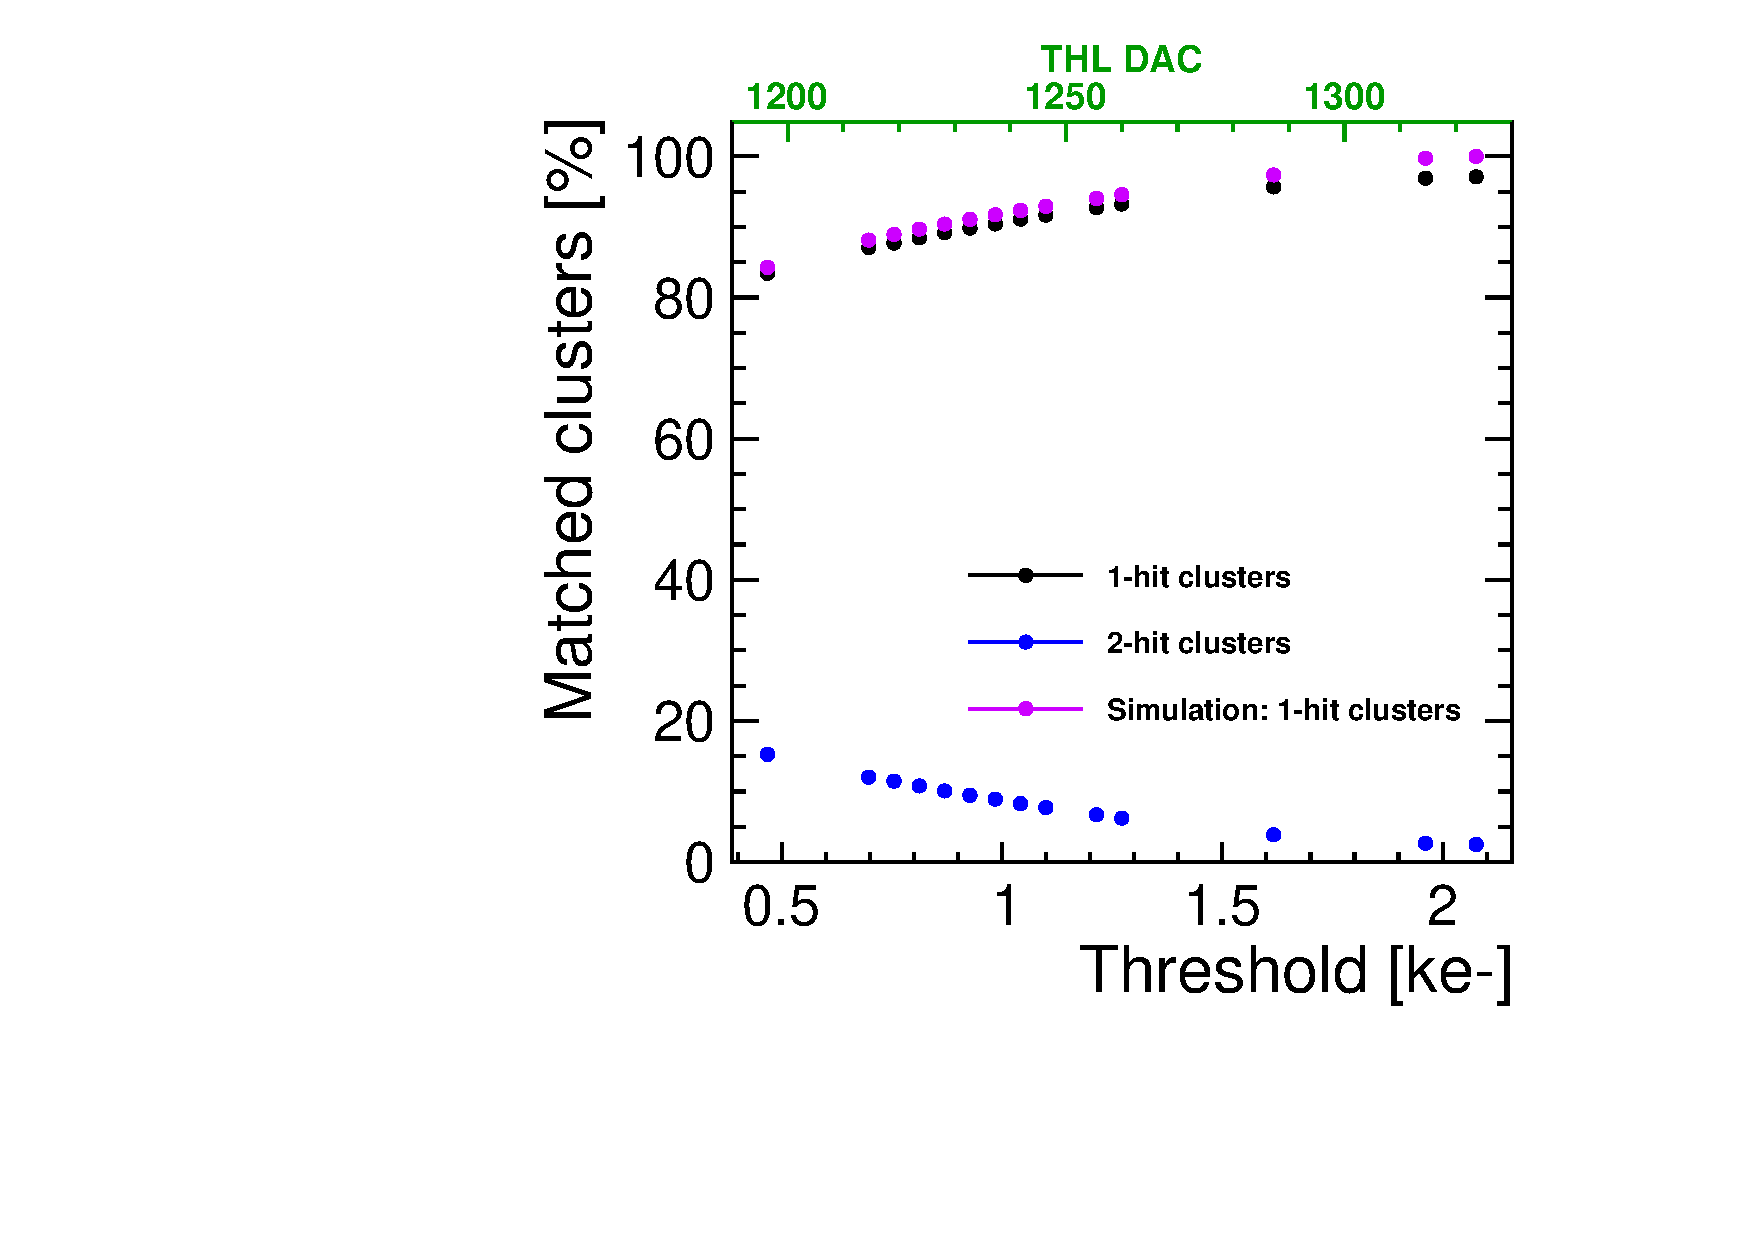
\includegraphics[width=\textwidth]{./figures/TestBeam/ThresholdScan_W0019_G07.pdf}
    \caption{}
  \end{subfigure} \hfill
  \begin{subfigure}[b]{0.45\textwidth}
    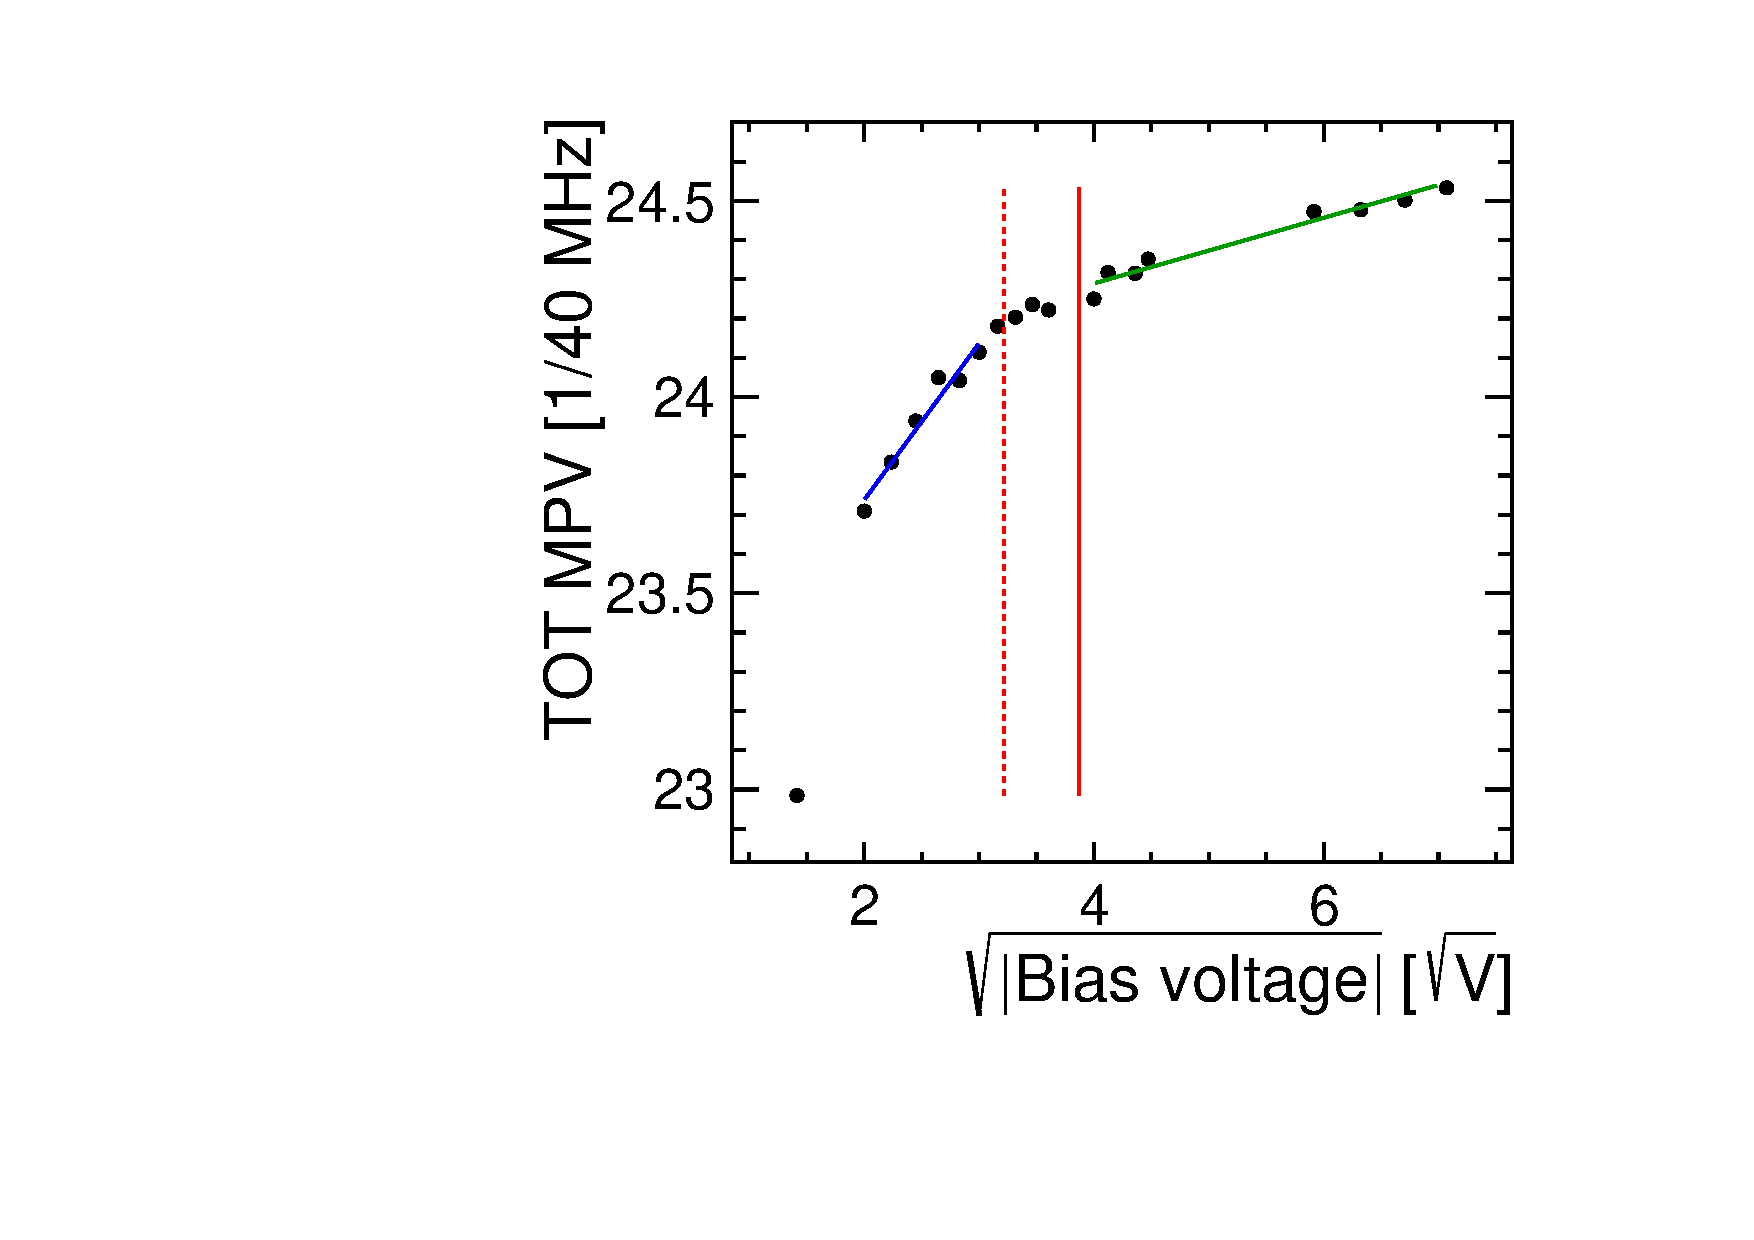
\includegraphics[width=\textwidth]{./figures/TestBeam/depletionVoltage_W0019_G07.pdf}
    \caption{}
  \end{subfigure}
  \caption{20-NGR (W19\_G7): bias and voltage scan.}
  \label{fig:Timepix3_THLscan_Vdep_G7}
\end{figure}

\begin{figure}[htbp] \centering
  \begin{subfigure}[b]{0.45\textwidth}
    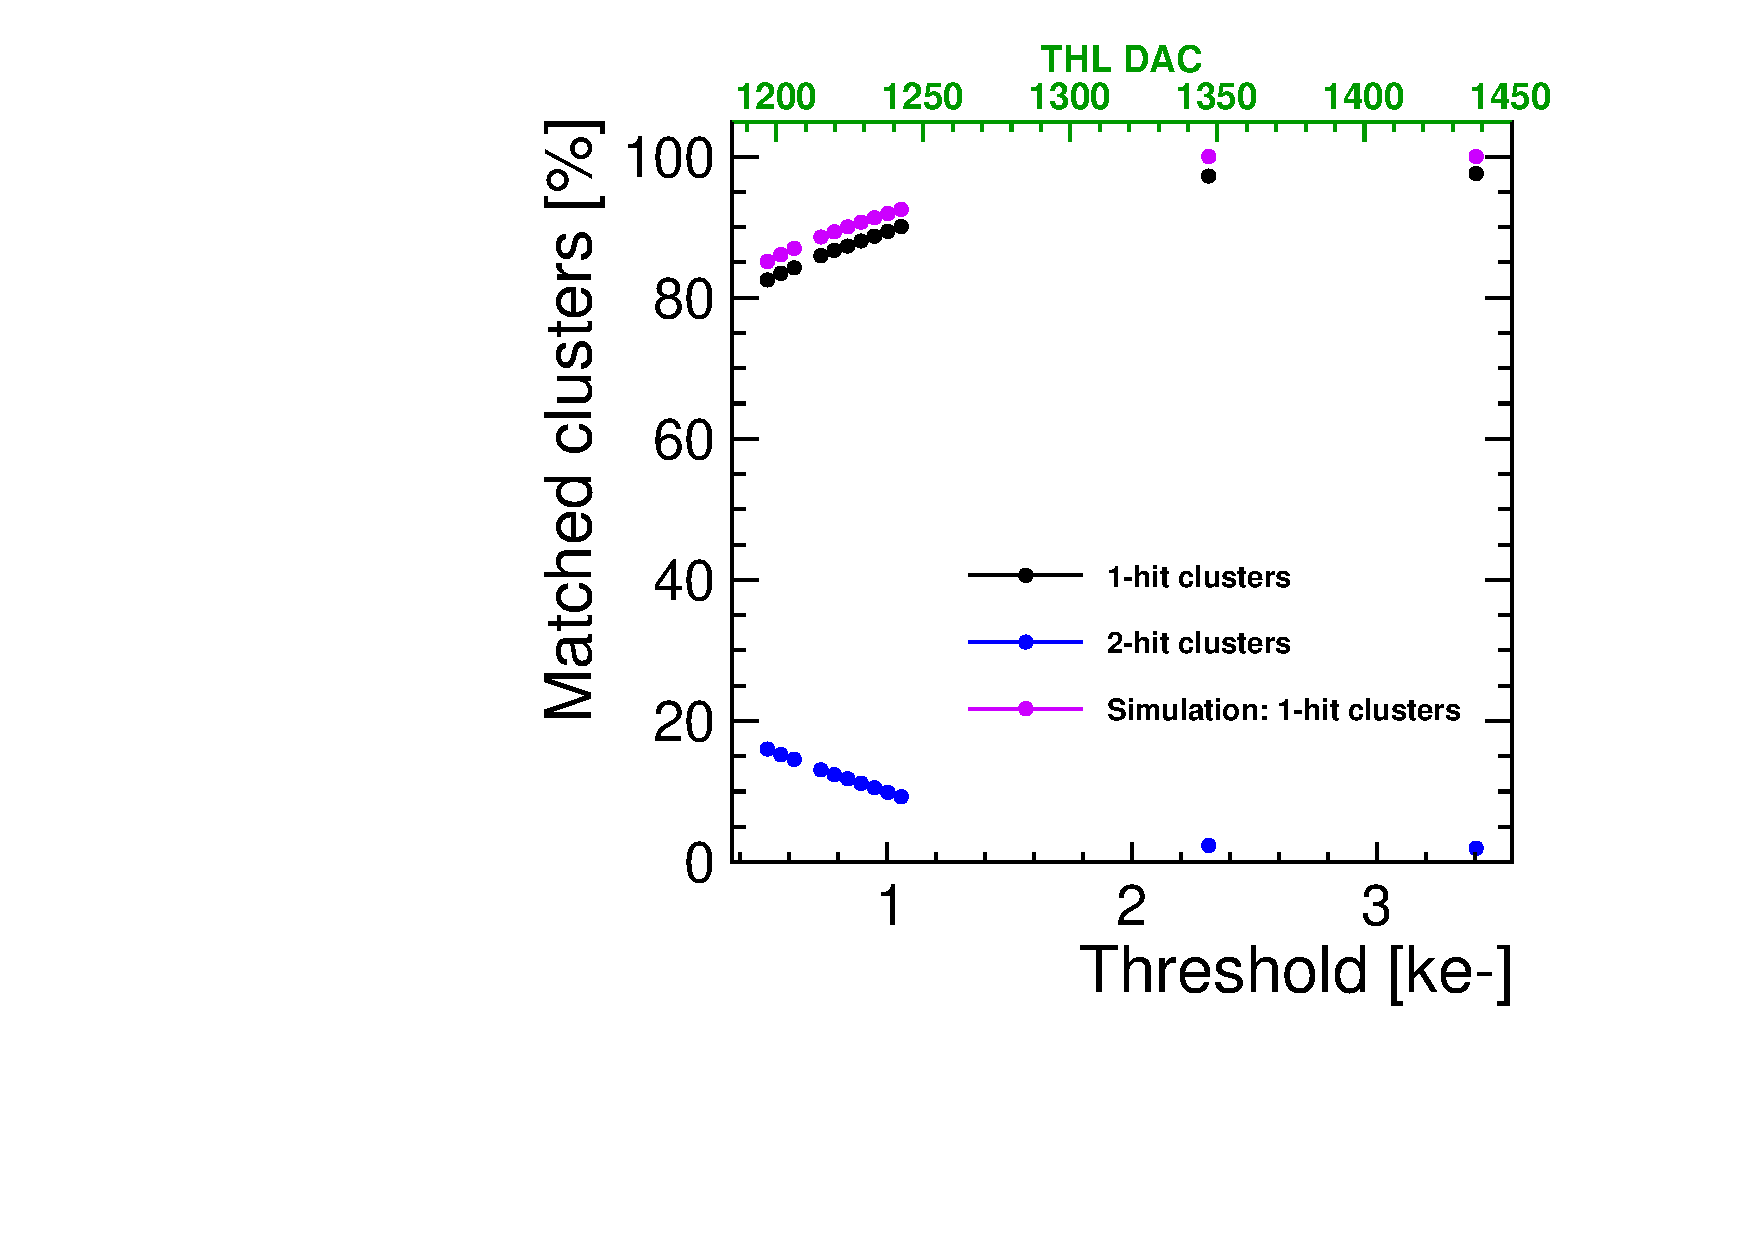
\includegraphics[width=\textwidth]{./figures/TestBeam/ThresholdScan_W0019_F07.pdf}
    \caption{}
  \end{subfigure} \hfill
  \begin{subfigure}[b]{0.45\textwidth}
    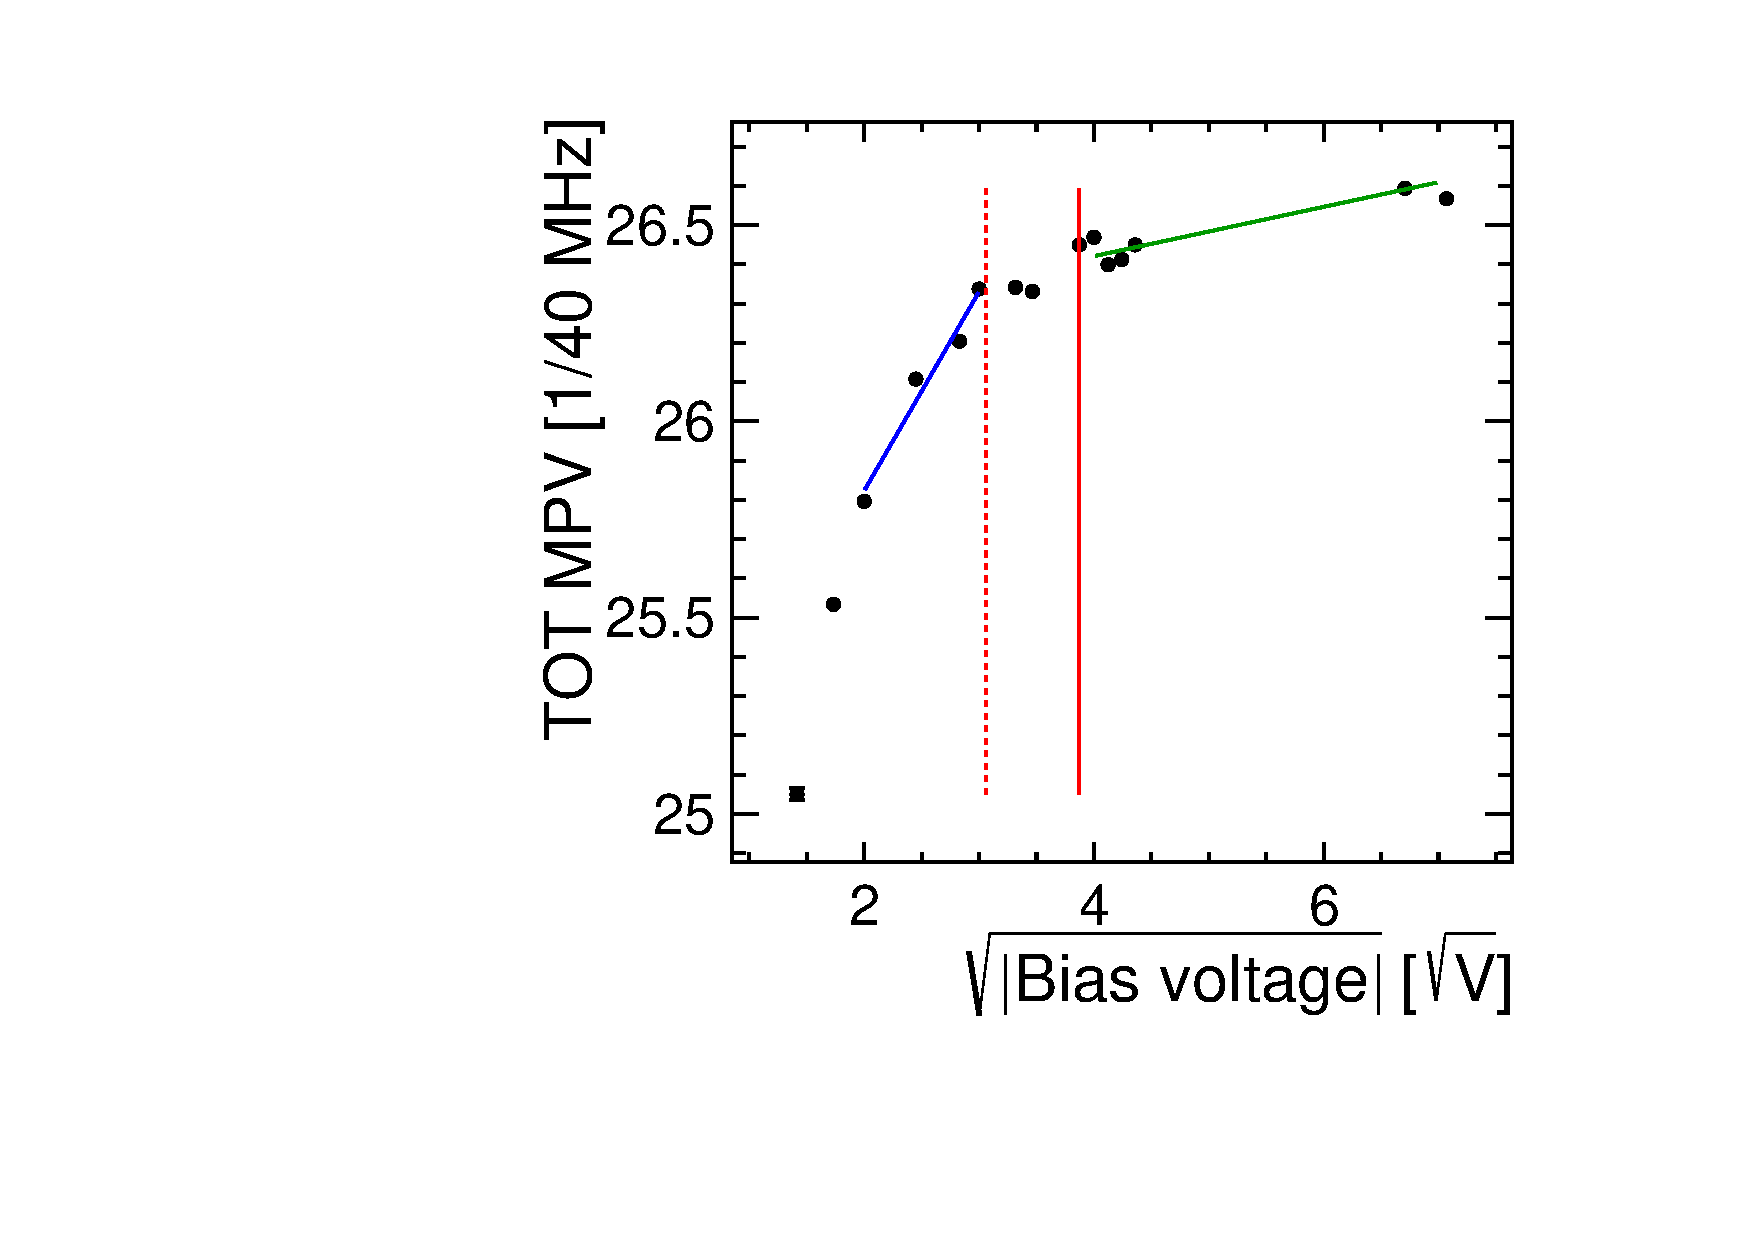
\includegraphics[width=\textwidth]{./figures/TestBeam/depletionVoltage_W0019_F07.pdf}
    \caption{}
  \end{subfigure}
  \caption{23-FGR (W19\_F7): bias and voltage scan.}
  \label{fig:Timepix3_THLscan_Vdep_F7}
\end{figure}

\begin{figure}[htbp] \centering
  \begin{subfigure}[b]{0.45\textwidth}
    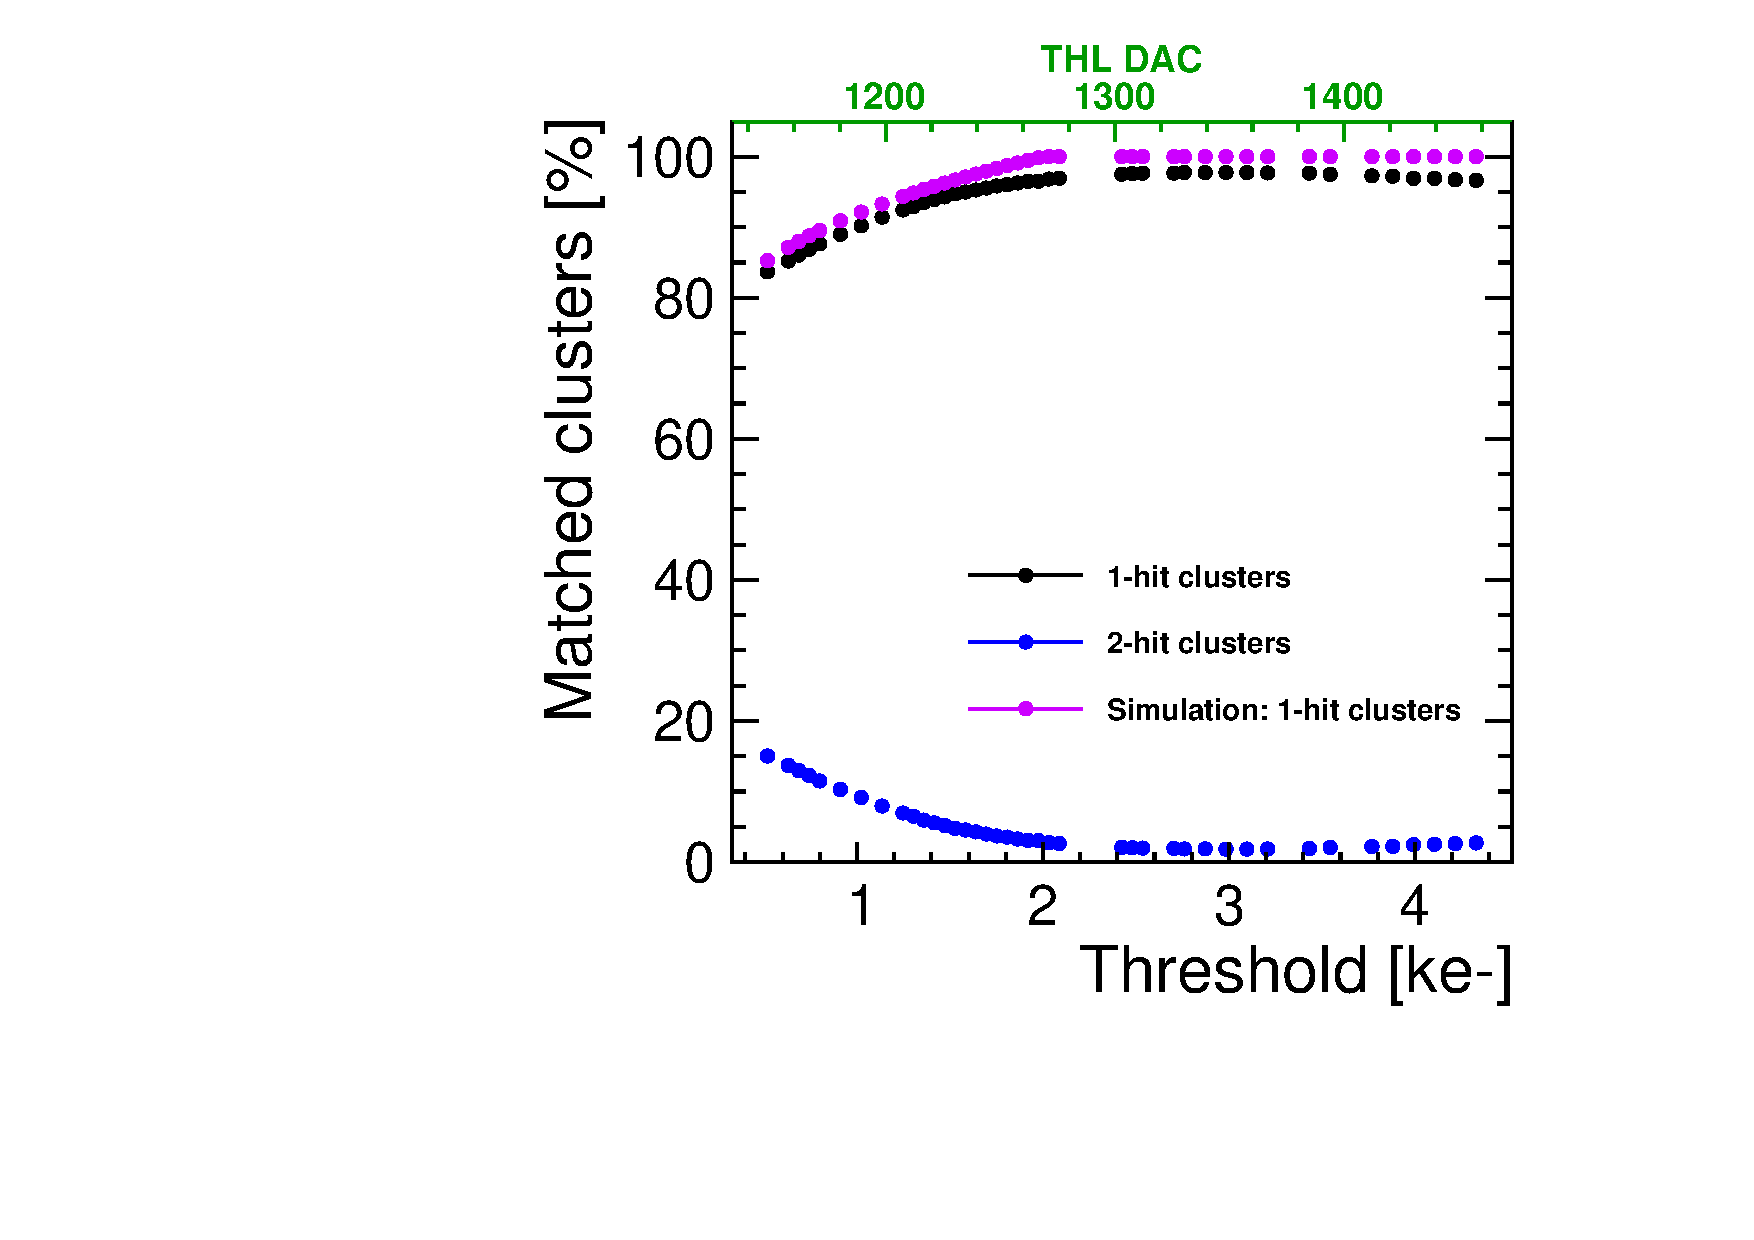
\includegraphics[width=\textwidth]{./figures/TestBeam/ThresholdScan_W0019_L08.pdf}
    \caption{}
  \end{subfigure} \hfill
  \begin{subfigure}[b]{0.45\textwidth}
    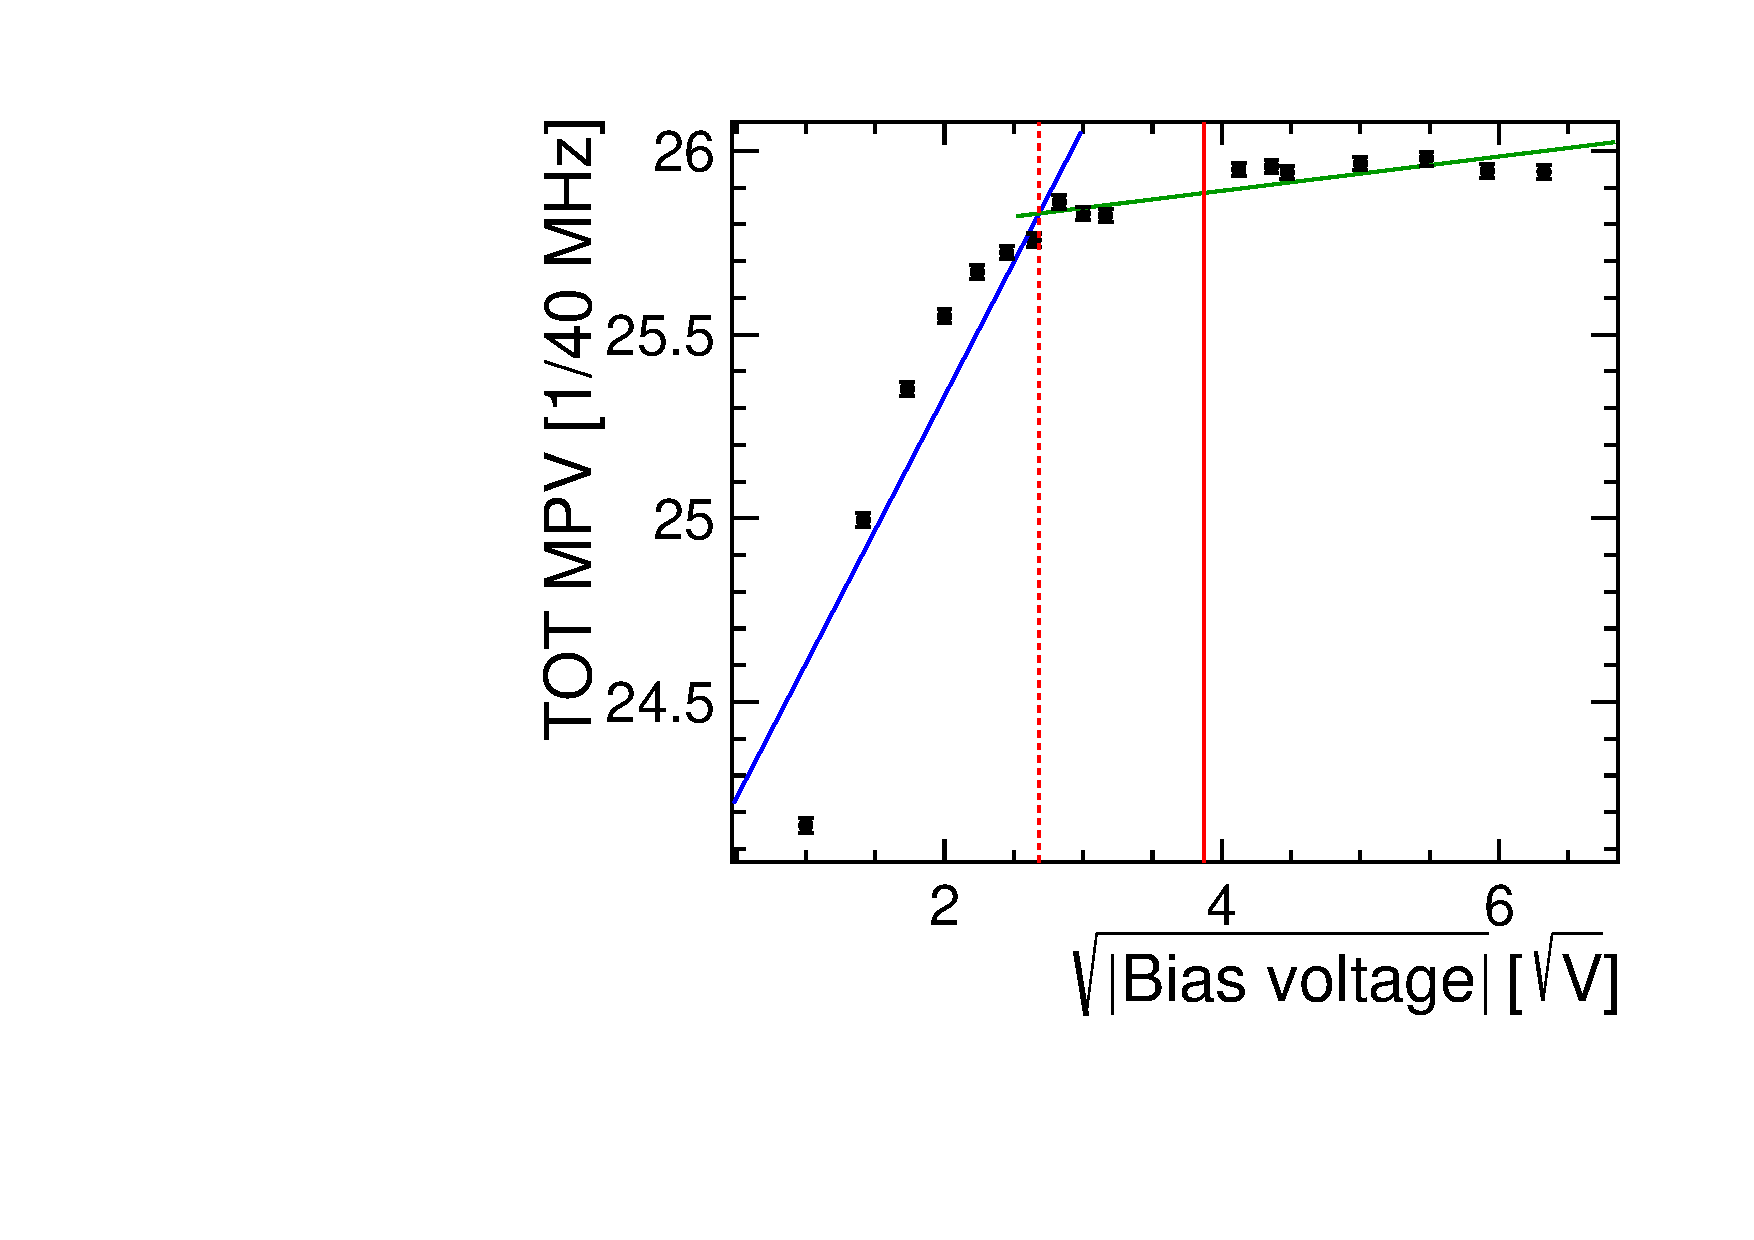
\includegraphics[width=\textwidth]{./figures/TestBeam/depletionVoltage_W0019_L08.pdf}
    \caption{}
  \end{subfigure}
  \caption{28-GNDGR (W19\_L8): bias and voltage scan.}
  \label{fig:Timepix3_THLscan_Vdep_L8}
\end{figure}


\begin{figure}[htbp] \centering
  \begin{subfigure}[b]{0.45\textwidth}
    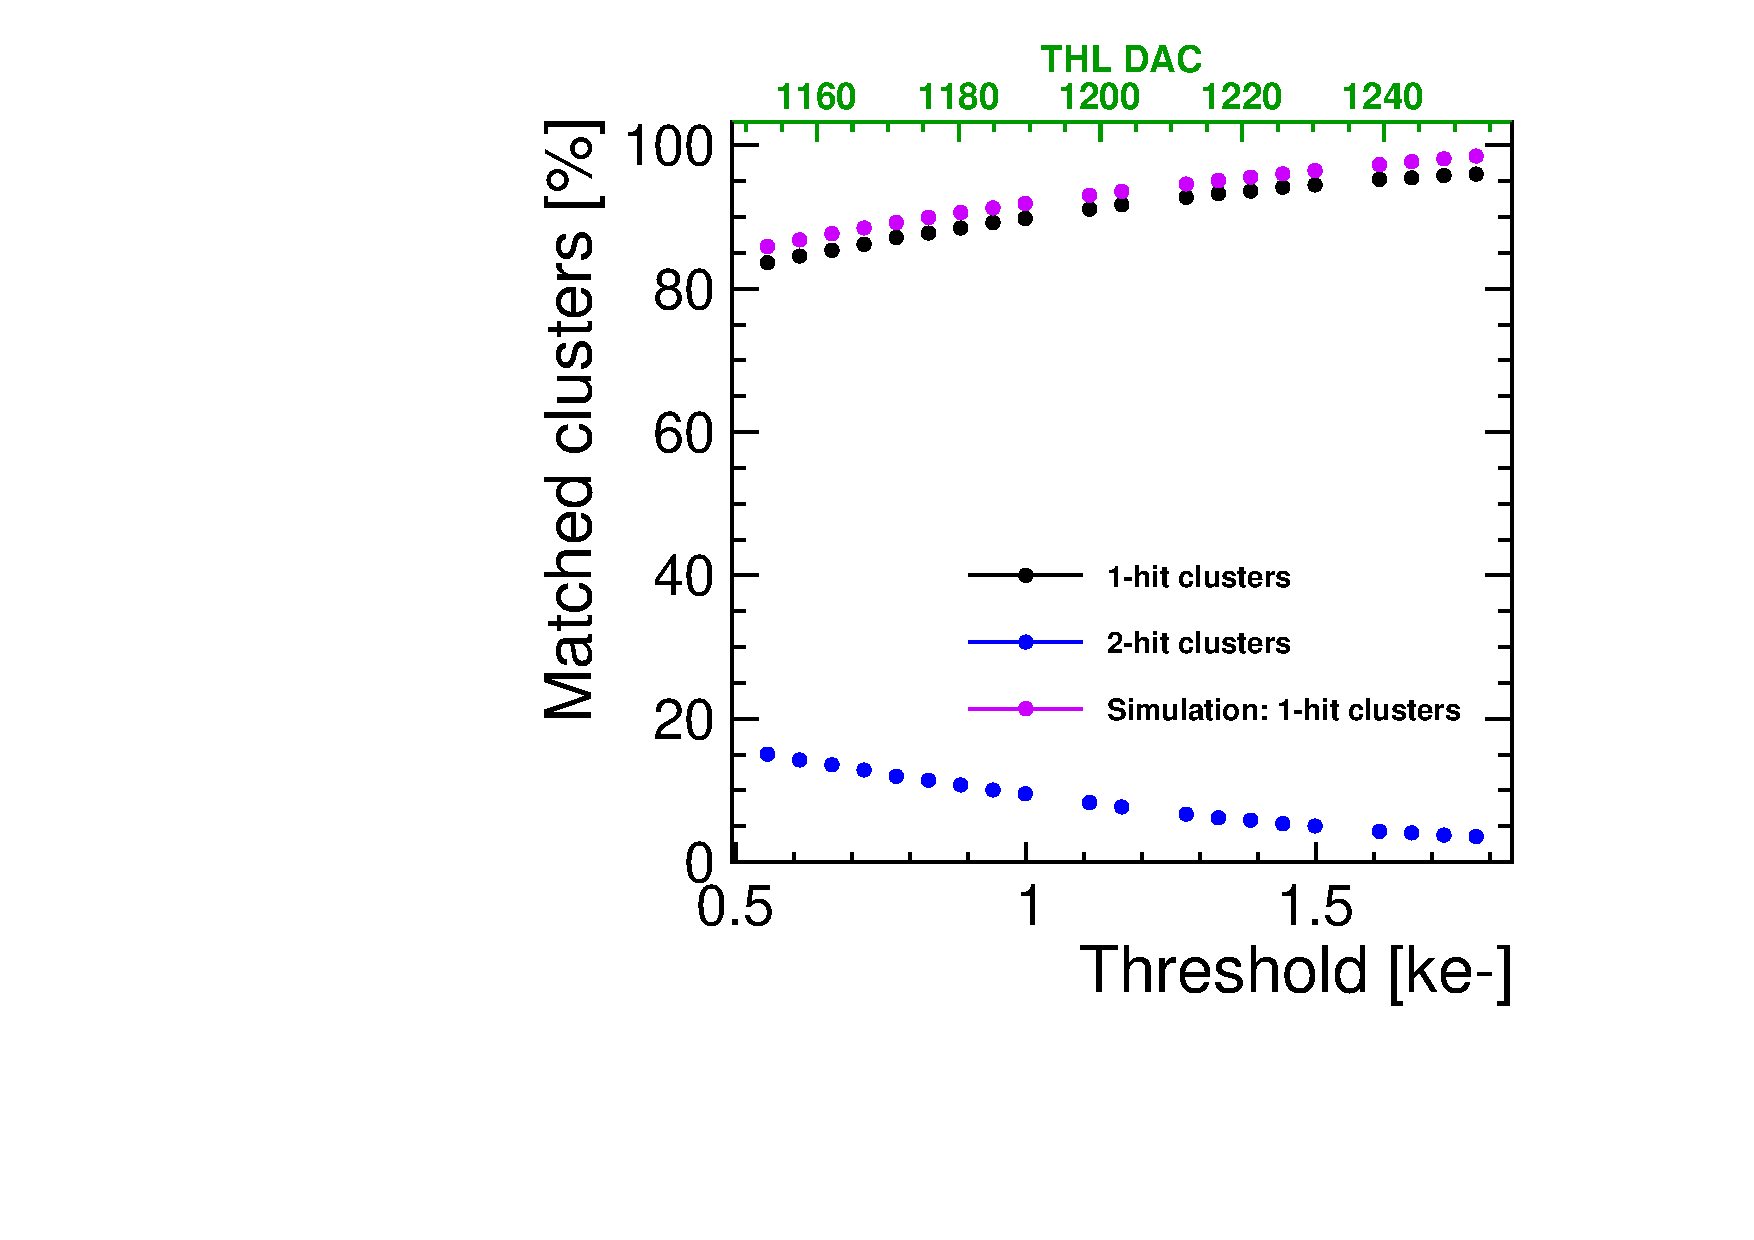
\includegraphics[width=\textwidth]{./figures/TestBeam/ThresholdScan_W0019_C07.pdf}
    \caption{}
  \end{subfigure} \hfill
  \begin{subfigure}[b]{0.45\textwidth}
    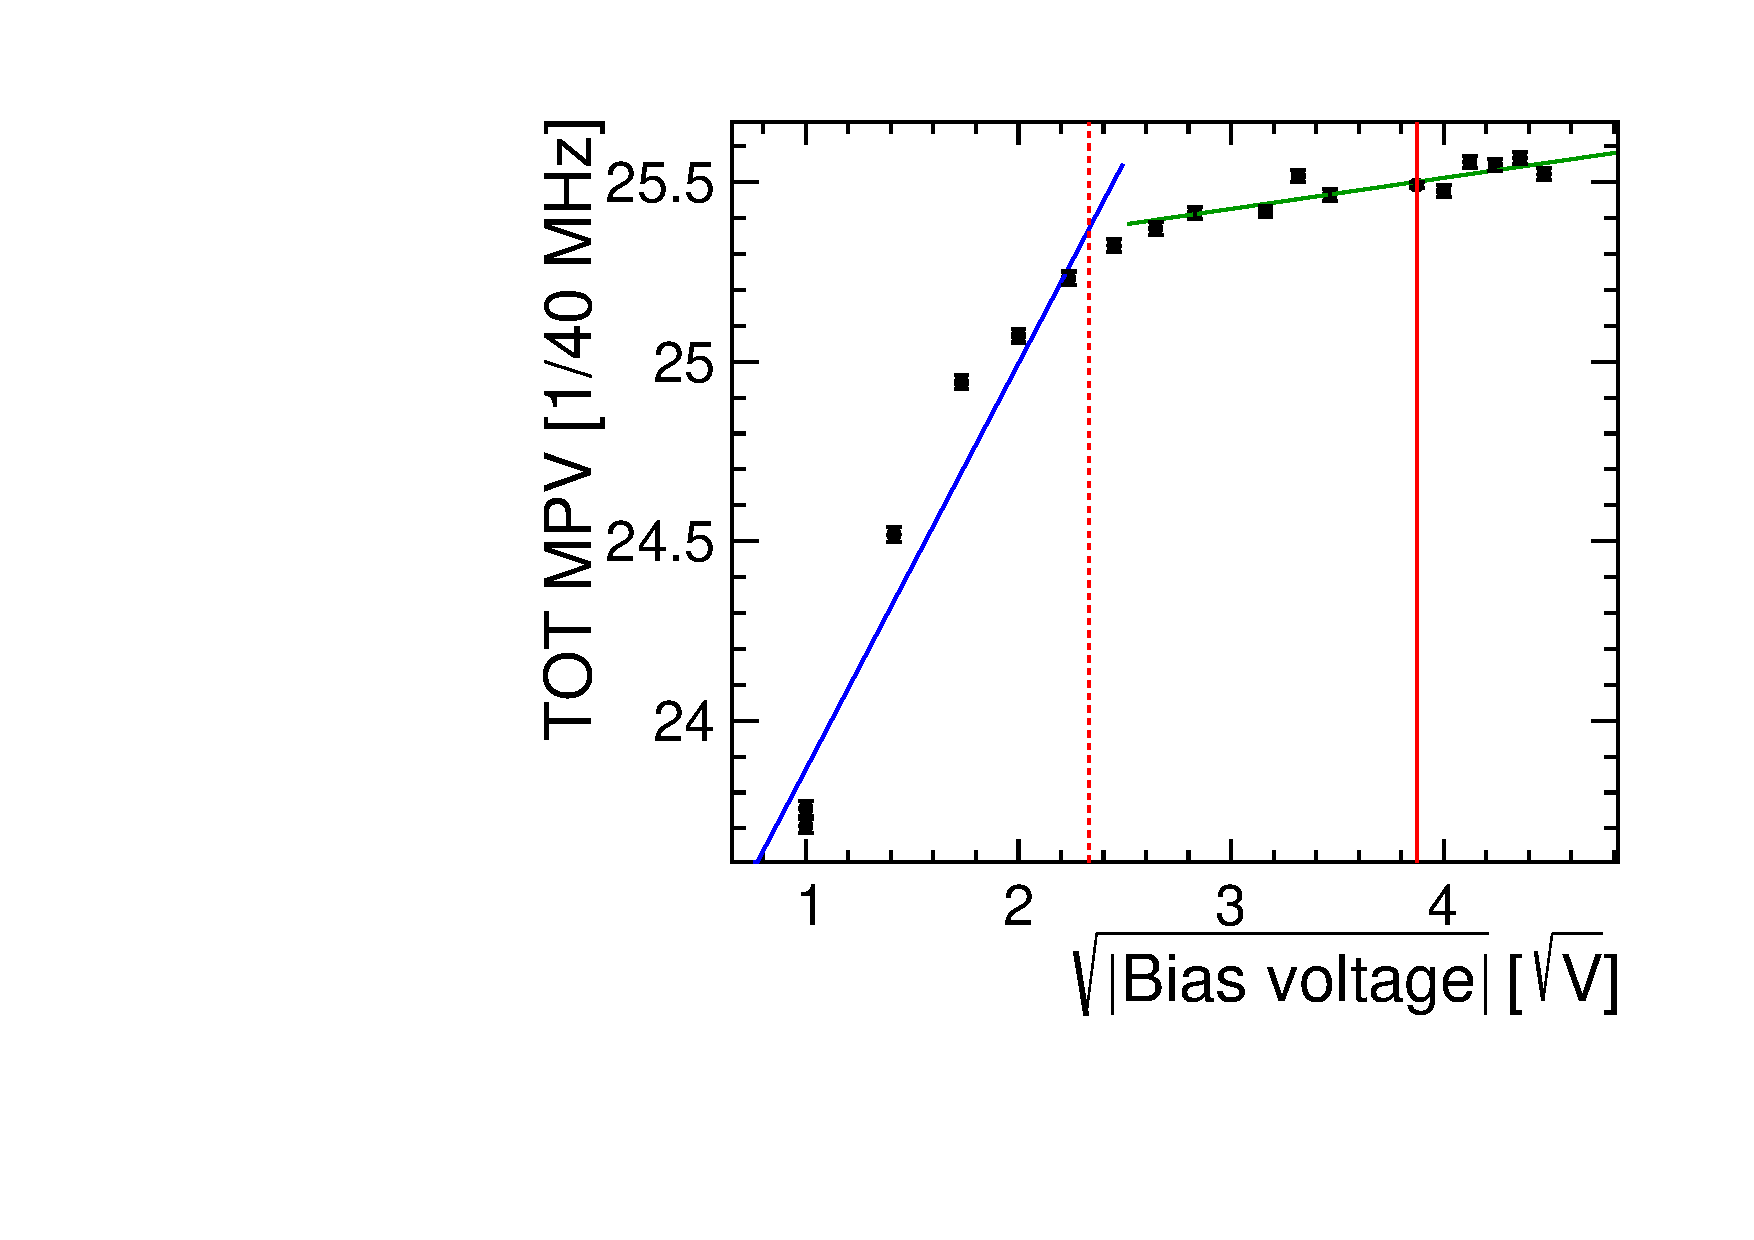
\includegraphics[width=\textwidth]{./figures/TestBeam/depletionVoltage_W0019_C07.pdf}
    \caption{}
  \end{subfigure}
  \caption{55-GNDGR (W19\_C7): bias and voltage scan.}
  \label{fig:Timepix3_THLscan_Vdep_C7}
\end{figure}

\begin{figure}[htbp] \centering
  \begin{subfigure}[b]{0.45\textwidth}
    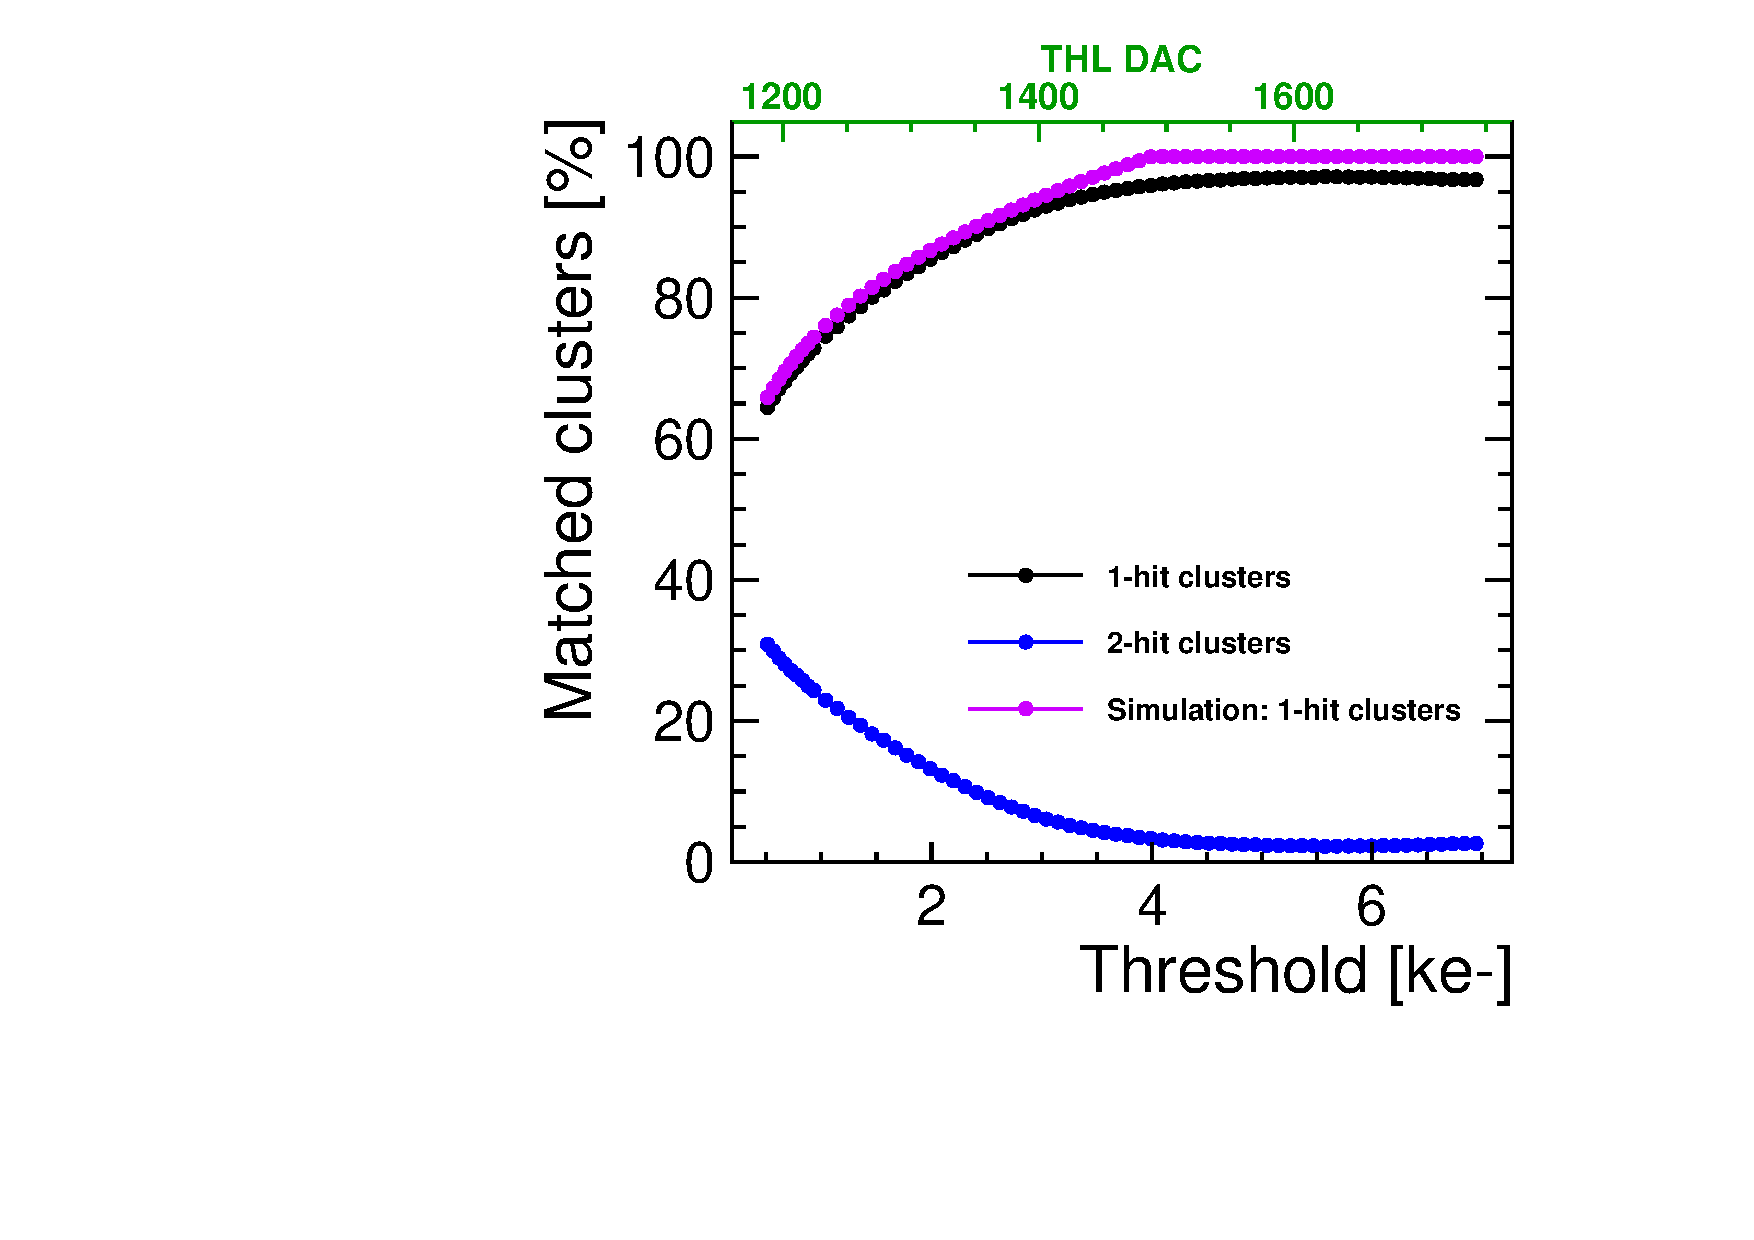
\includegraphics[width=\textwidth]{./figures/TestBeam/ThresholdScan_W0005_E02.pdf}
    \caption{}
  \end{subfigure} \hfill
  \begin{subfigure}[b]{0.45\textwidth}
%    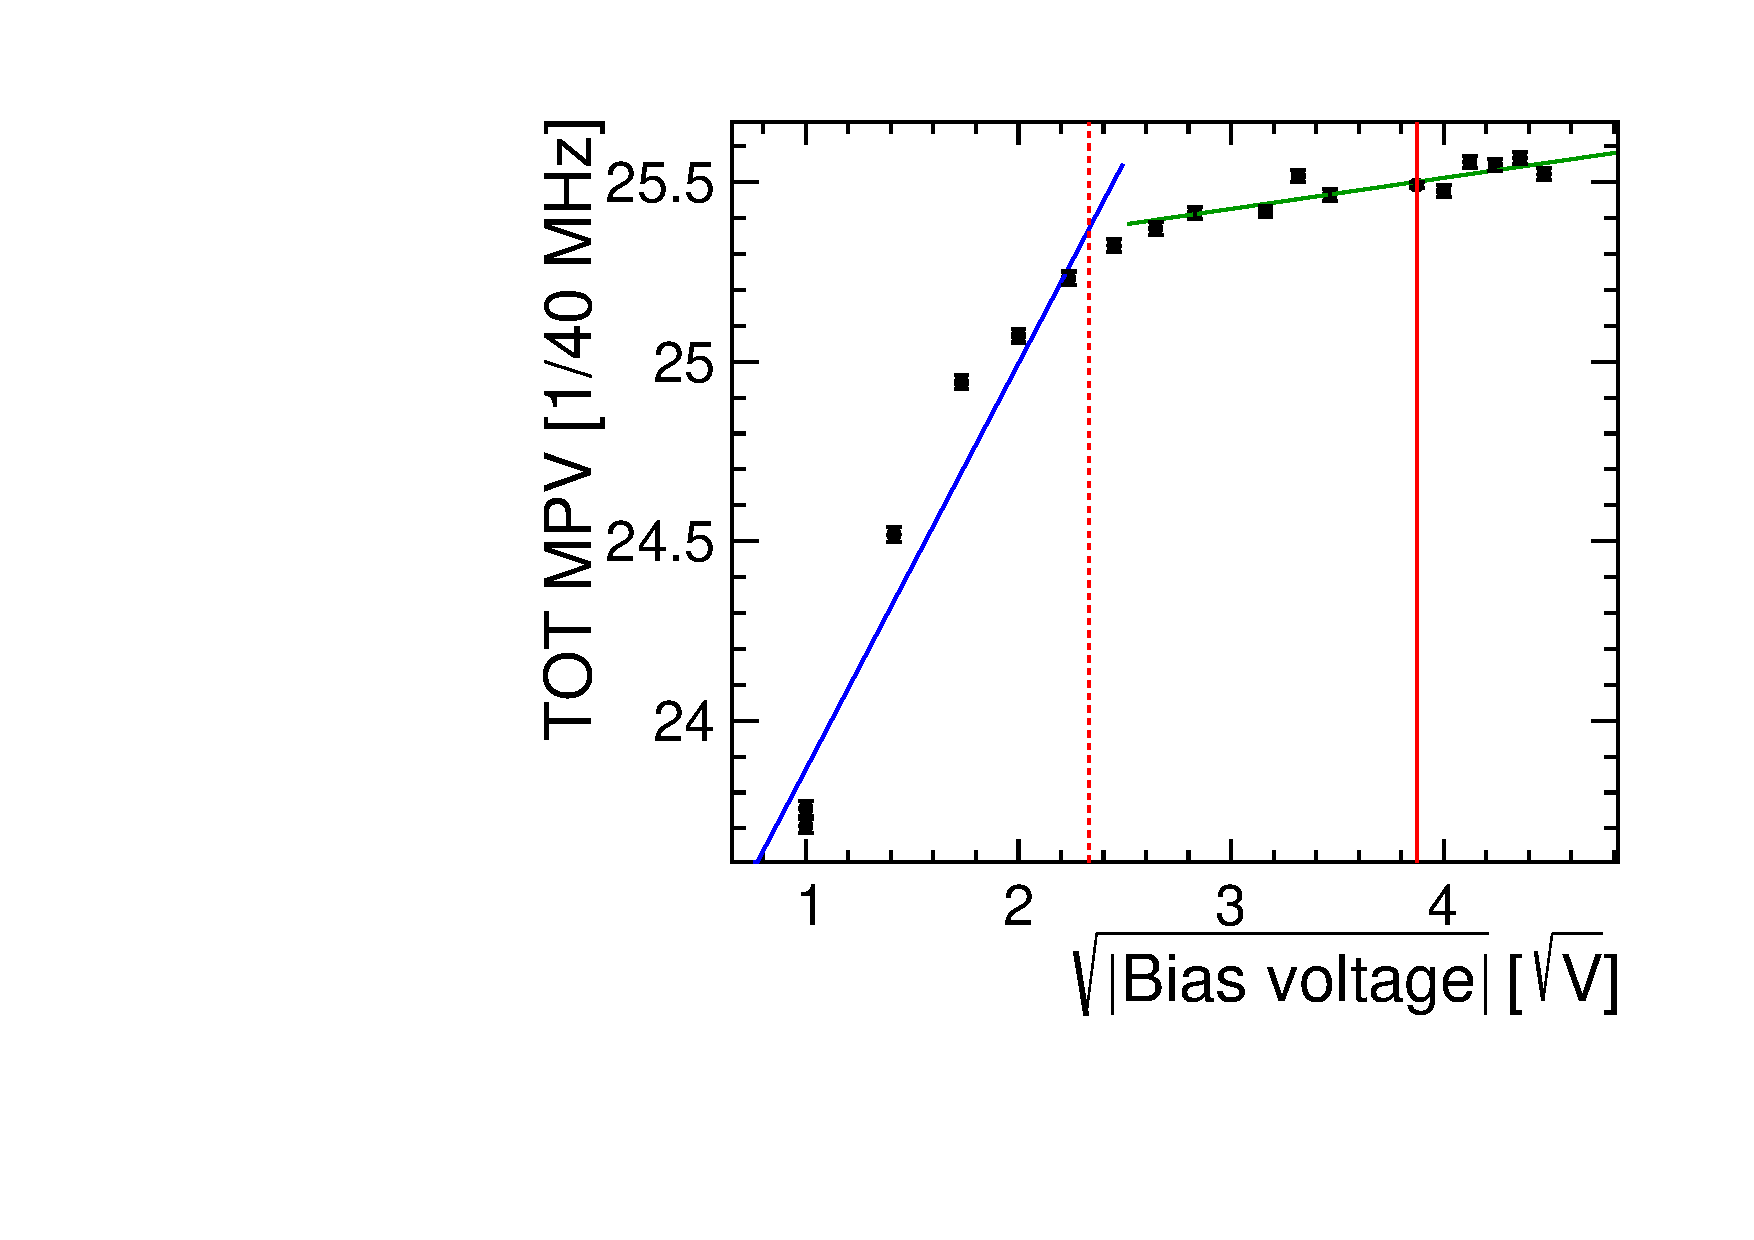
\includegraphics[width=\textwidth]{./figures/TestBeam/depletionVoltage_W0019_C07.pdf}
    \caption{}
  \end{subfigure}
  \caption{55-GNDGR-100 (W5\_E2): bias and voltage scan.}
  \label{fig:Timepix3_THLscan_Vdep_E2}
\end{figure}


\begin{figure}[htbp] \centering
  \begin{subfigure}[b]{0.45\textwidth}
    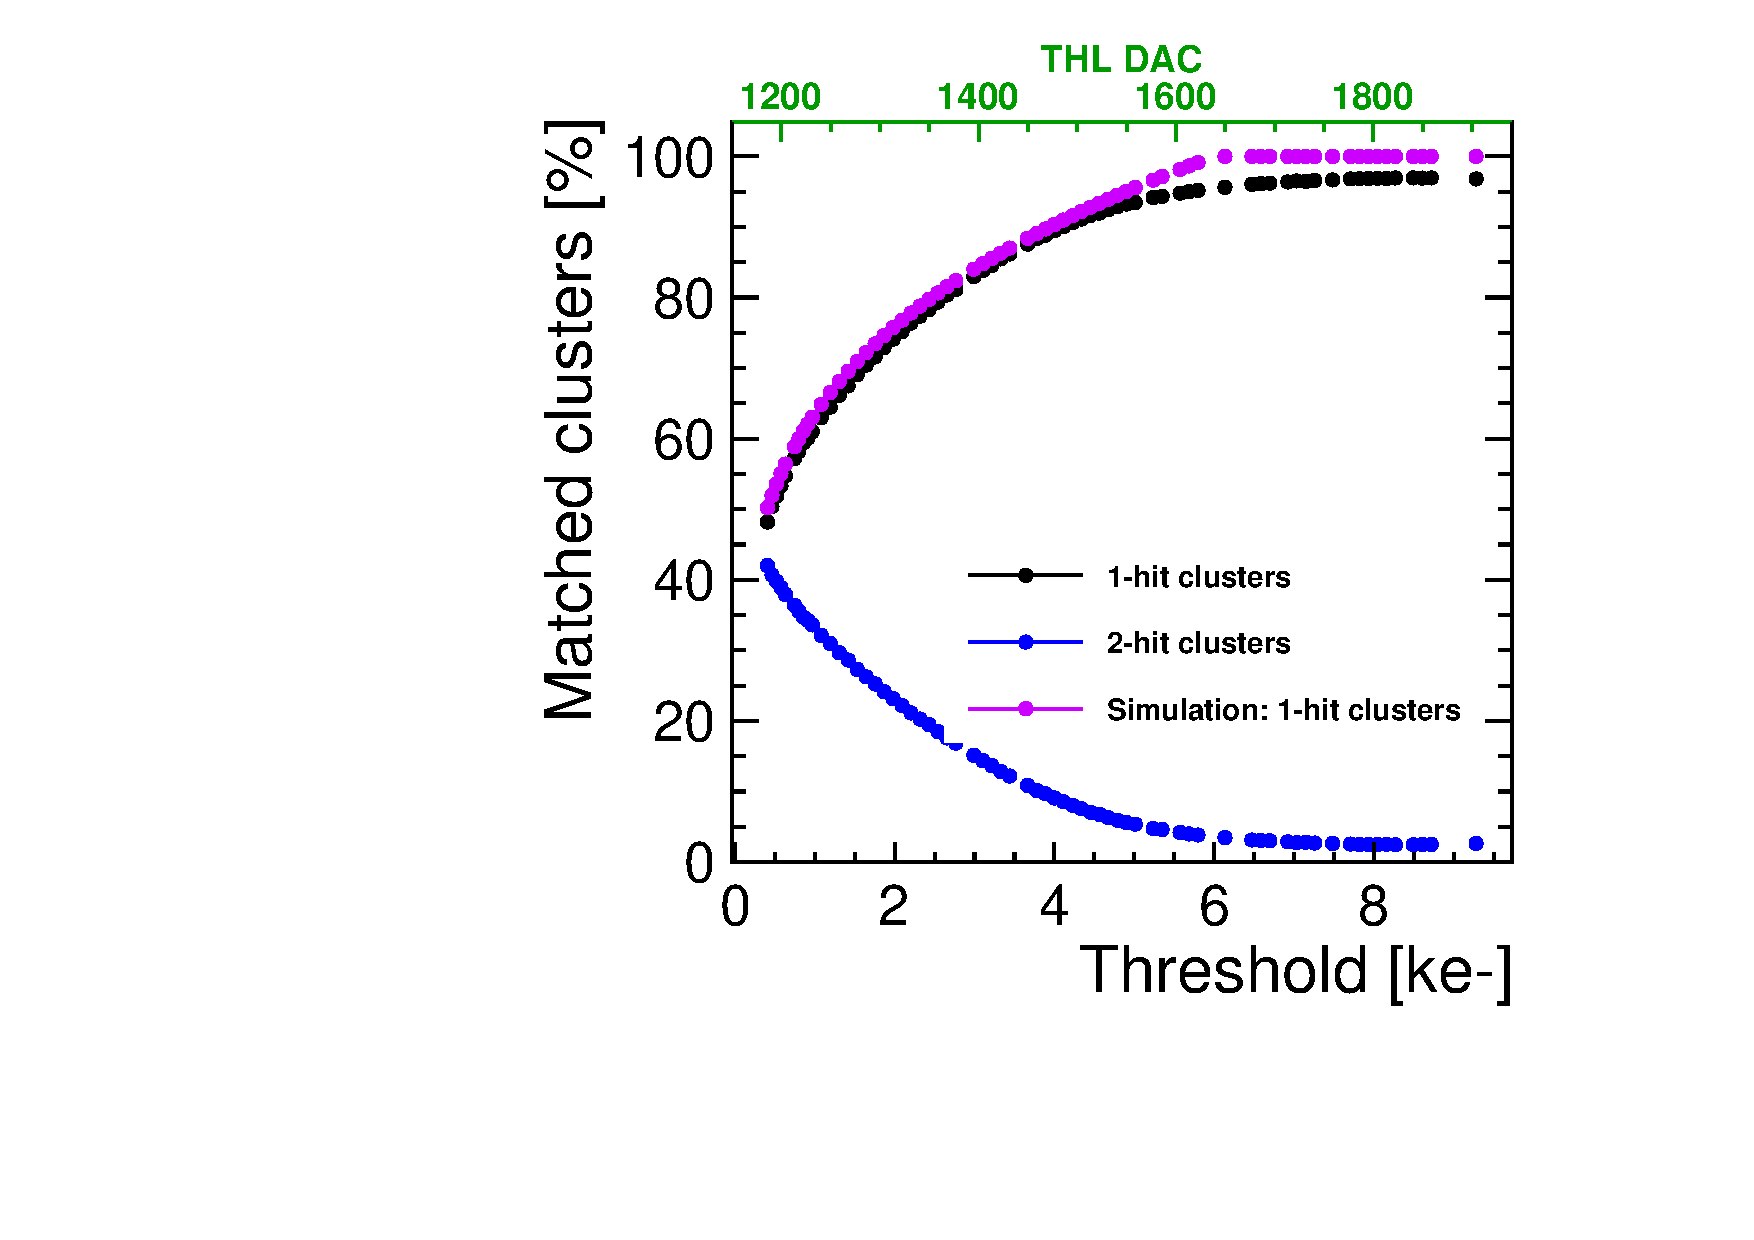
\includegraphics[width=\textwidth]{./figures/TestBeam/ThresholdScan_W0005_F01.pdf}
    \caption{}
  \end{subfigure} \hfill
  \begin{subfigure}[b]{0.45\textwidth}
    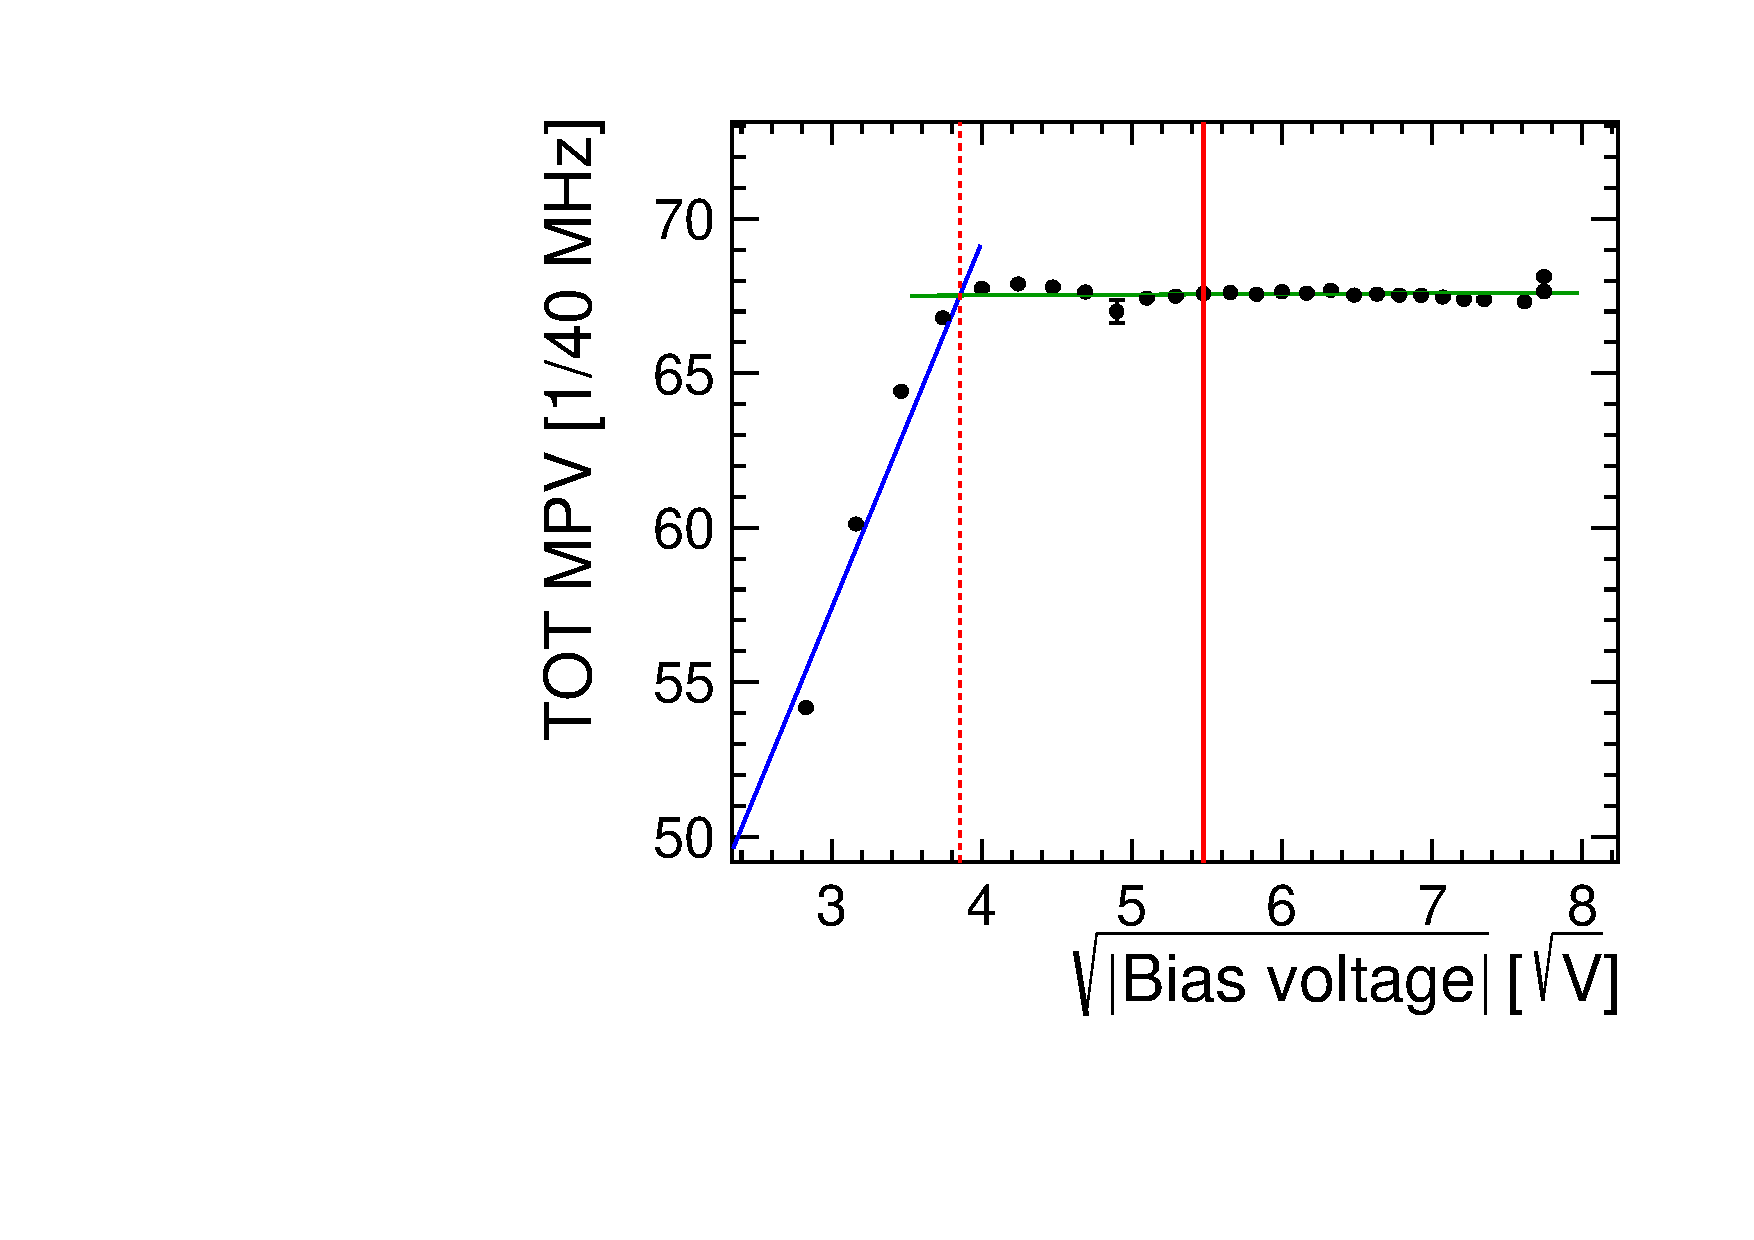
\includegraphics[width=\textwidth]{./figures/TestBeam/depletionVoltage_W0005_F01.pdf}
    \caption{}
  \end{subfigure}
  \caption{55-GNDGR-150 (W5\_F1): bias and voltage scan.}
  \label{fig:Timepix3_THLscan_Vdep_F1}
\end{figure}
